\paragraph{Osteosynthesis plates}

\begin{figure}[ht]
    \centering
    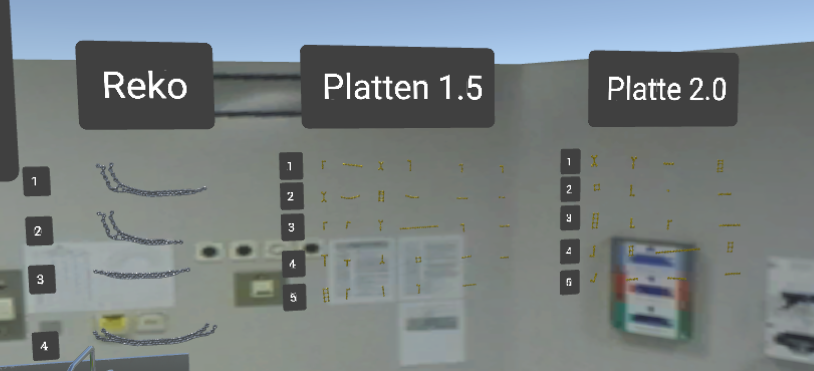
\includegraphics[width=200px]{images/implementation/features/procedures/metal_plates_1.png}
    \caption{\label{fig::FeatureMetalPlate} Over view of all available steosynthesis plates. Users can choose from four reconstructional plates, 29 1.5mm plates and 20 2mm plates to apply in the procedure.}
\end{figure}

The \textbf{osteosynthesis plates} procedure consists of two steps before adding it as a step to the project case.
First, users have to chose which plate to use.
The user can chose from four reconstruction plates, 29 1.5mm plates and 20 2.0mm plates (Figure \ref{fig::FeatureMetalPlate}).
The optimal plates to use vary due to the pathology of the patient and the previously performed procedures.
After selecting the proper plate, a number of indicators will show to the user (Figure \ref{fig::FeatureMetalPlate2}).

\begin{figure}
  \centering
  \begin{minipage}{.5\textwidth}
    \centering
    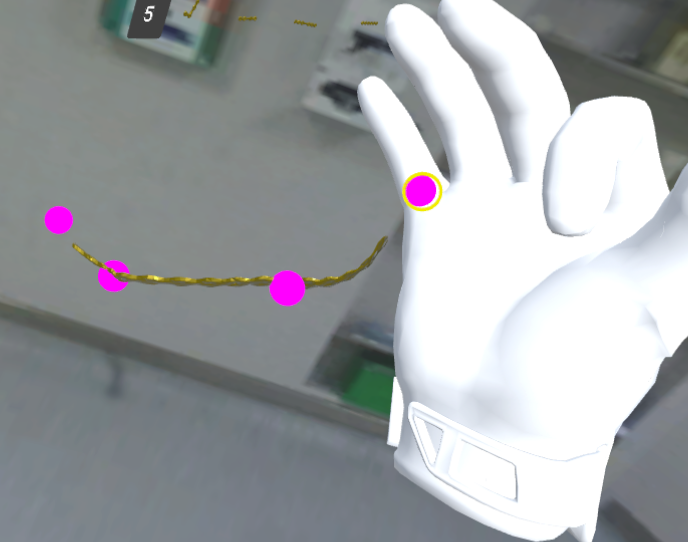
\includegraphics[width=0.95\linewidth]{images/implementation/features/procedures/metal_plates_2.png}
  \end{minipage}%
  \begin{minipage}{.5\textwidth}
    \centering
    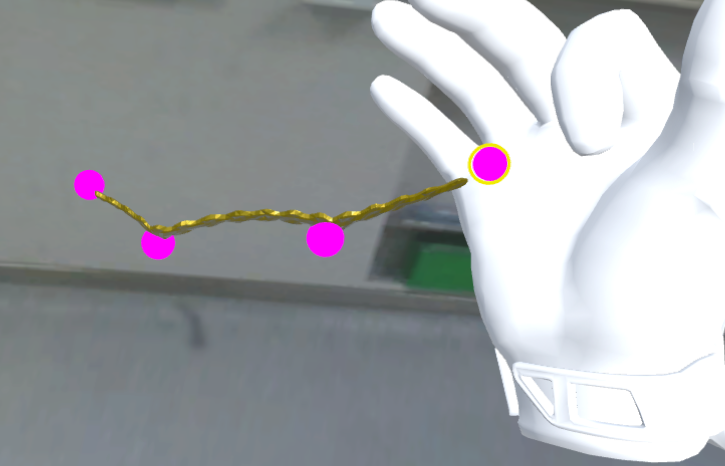
\includegraphics[width=0.95\linewidth]{images/implementation/features/procedures/metal_plates_3.png}
  \end{minipage}
  \caption{\label{fig::FeatureMetalPlate2}Osteosynthesis Plates Modifications. User can translate and rotate control points to perform modifications to the plates shape} 
\end{figure}

In the context of the osteosynthesis plates, these indicators are "control points", with which the user can bend and twist the plates.
These control points were set manually according to each of the osteosynthesises plates after investigating how different amounts of control points would affect the geometry.
The control points act as knots in a spline based calculation of the geometries mesh.
Bending and twisting is performed by choosing a control point via hovering over them with the user's free hand and grabbing them.
Then, the user has to move and rotate the control point in the desired manner (Figure \ref{fig::FeatureMetalPlate2}).
